\subsubsection{DfuSe Programm}
\label{sec:DFUSe}

STMicroelectronics stellt eine Software namens DfuSe zur Verfügung um die Firmware STM32 Devices ohne Debugger zu programmieren. Siehe Kapitel \ref{sec:KeilInstall} für die Installation des DfuSe Tools.

\paragraph{HEX File zu DFU File konvertieren}

Für den Prozess verlangt das Tool, ein \texttt{.dfu} Dateiformat, dass nicht von der IDE erzeugt wird. 
Im Normalfall ist die kompilierte Binärdatei aus Keil uVision 5 im \texttt{.hex} Format im Projektordner unter \texttt{./MDK-ARM/<Projektname>/<Projektname>.hex} zu finden.\\

Das DfuSe Tool kommt mit einem weiteren Werkzeug, um Dateien vom \texttt{.hex} ins \texttt{.dfu} Format zu konvertieren. 
Dieses heisst DFU File Manager und ist in Abbildung \ref{pic:DFU_file_man} dargestellt.

\begin{figure}[H]
	\centering
	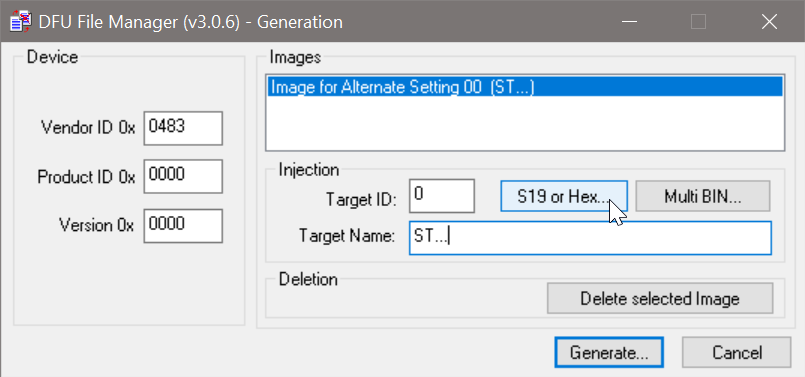
\includegraphics[width=0.5\linewidth]{DFU_file_man}
	\caption{Firmware Upgrade Tool DfuSe}
	\label{pic:DFU_file_man}
\end{figure}

Den DFU File Manager starten und \glqq\textit{I want to GENERATE a DFU file from HEX}\grqq \ auswählen.
Darauf präsentiert sich das Tool wie in Abbildung \ref{pic:DFU_file_man}. Hier kann eine \texttt{.hex} Datei ausgewählt und anschliessend konvertiert und gespeichert werden.
Mit Klick auf \textit{\glqq S19 or HEX...\grqq} kann das \texttt{<Projektname>.hex} ausgewählt und anschliessend mit Klick auf \textit{\glqq Generate...\grqq} ein \texttt{<Projektname>.dfu} generiert werden.
\\
\paragraph{DFU Datei auf das DSP Board laden}\vspace{-0.3cm}\\
Die nun erstellte \texttt{<Projektname>.dfu} Datei kann mit dem DfuSe Programm auf das im DFU Modus gebootete DSP-Board programmiert werden. 
Die Abbildung \ref{pic:DFUSe_Upgrade} zeigt das DfuSe Programm, bei dem das DSP-Board bereits am USB Port erkannt wurde. Die Erkennung geschieht automatisch, sofern das DSP-Board über USB am Computer angeschlossen ist und sich im Bootloader befindet.

\begin{figure}[H]
	\centering
	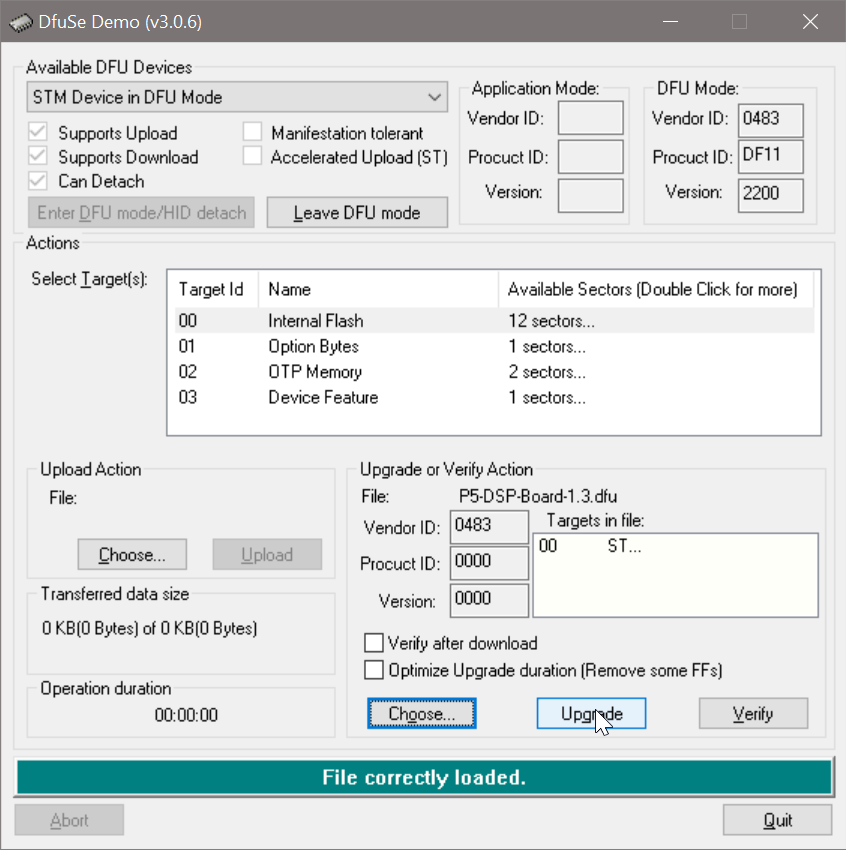
\includegraphics[width=0.65\linewidth]{DFUSe_Upgrade}
	\caption{Firmware Upgrade Tool DfuSe}
	\label{pic:DFUSe_Upgrade}
\end{figure}

Mit Klick auf \textit{\glqq Choose...\grqq} wird die \texttt{<Projektname>.dfu} ausgewählt.
Anschliessend mit \glqq\textit{Upgrade}\grqq \ die neue Firmware programmieren.
Dabei erscheint eine Warnung \textit{\glqq ...it is impossible to make sure this file is for device.\grqq}, welche mit \textit{\glqq Yes\grqq} bestätigt werden kann.

Wenn das Upgrade vollzogen ist, erscheint der Balken unten in grün. Jetzt kann das DSP-Board mit \textit{\glqq Leave DFU Mode\grqq} neu gestartet werden.


